\documentclass[a4paper]{article}

\usepackage{tikz}
\usetikzlibrary{positioning, arrows.meta, shapes, calc}
\usepackage{float}
\usepackage{geometry}
\geometry{margin=1.5cm, landscape}

\begin{document}

\title{System Overview: Nuevo Pipeline Architecture}
\author{}
\date{}
\maketitle

\section{System Overview}

This diagram illustrates the detailed architecture of the \texttt{nuevo} pipeline, showing internal processing steps and data flows for both main components.

\begin{figure}[H]
  \centering
  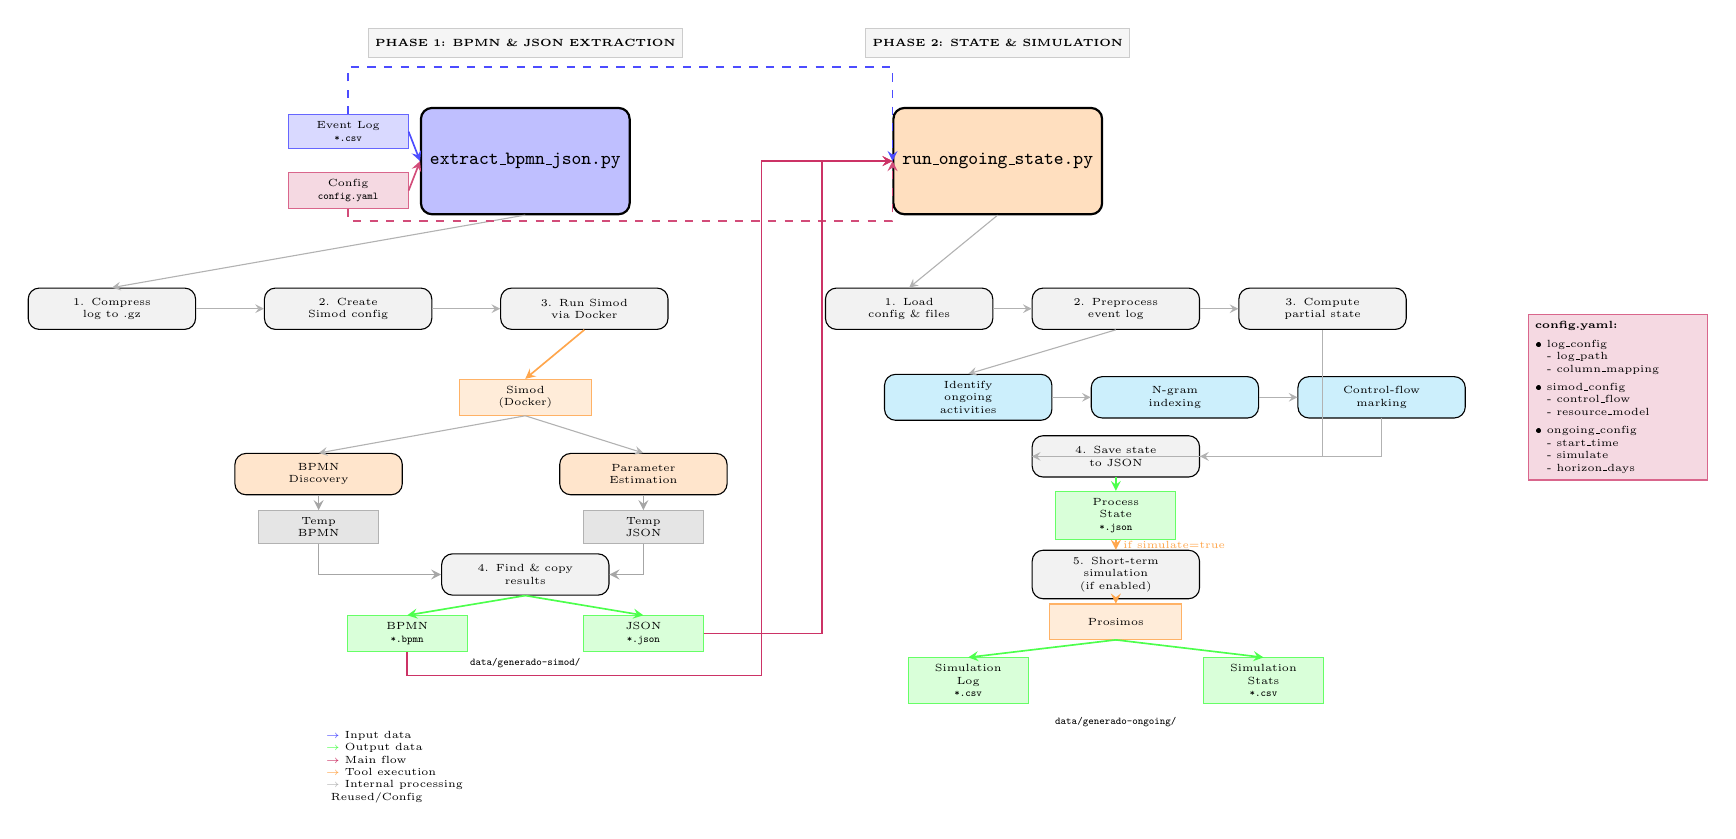
\begin{tikzpicture}[
    scale=0.75,
    transform shape,
    node distance=0.8cm and 1.5cm,
    script/.style={rectangle, rounded corners, draw=black, thick, 
                   minimum width=3.5cm, minimum height=1.8cm, 
                   text width=3.3cm, align=center, font=\small\bfseries},
    procstep/.style={rectangle, rounded corners, draw=black, fill=gray!10,
                 minimum width=2.8cm, minimum height=0.7cm,
                 text width=2.6cm, align=center, font=\tiny},
    input/.style={rectangle, draw=blue!60, fill=blue!15, 
                  minimum width=2cm, minimum height=0.5cm, 
                  text width=1.8cm, align=center, font=\tiny},
    output/.style={rectangle, draw=green!60, fill=green!15, 
                   minimum width=2cm, minimum height=0.5cm, 
                   text width=1.8cm, align=center, font=\tiny},
    config/.style={rectangle, draw=purple!60, fill=purple!15, 
                   minimum width=2cm, minimum height=0.5cm, 
                   text width=1.8cm, align=center, font=\tiny},
    tool/.style={rectangle, draw=orange!60, fill=orange!15,
                 minimum width=2.2cm, minimum height=0.6cm,
                 text width=2cm, align=center, font=\tiny},
    arrow/.style={->, >=stealth, semithick},
    phase/.style={rectangle, draw=gray!40, fill=gray!8, 
                  minimum width=3cm, minimum height=0.5cm, 
                  font=\tiny\bfseries, align=center},
    internal/.style={->, >=stealth, thin, gray!60}
  ]
    
    % Phase labels at top
    \node[phase] (phase1) at (-4, 7) {PHASE 1: BPMN \& JSON EXTRACTION};
    \node[phase] (phase2) at (4, 7) {PHASE 2: STATE \& SIMULATION};
    
    % ========== PHASE 1 DETAILS ==========
    
    % Inputs to Phase 1
    \node[input] (log) at (-7, 5.5) {Event Log\\\texttt{*.csv}};
    \node[config] (config) at (-7, 4.5) {Config\\\texttt{config.yaml}};
    
    % extract_bpmn_json.py main module
    \node[script, fill=blue!25] (extract) at (-4, 5) {
      \texttt{extract\_bpmn\_json.py}
    };
    
    % Internal steps of extract_bpmn_json.py
    \node[procstep] (compress) at (-11, 2.5) {1. Compress\\log to .gz};
    \node[procstep] (create-config) at (-7, 2.5) {2. Create\\Simod config};
    \node[procstep] (docker) at (-3, 2.5) {3. Run Simod\\via Docker};
    
    % Simod tool
    \node[tool] (simod) at (-4, 1) {Simod\\(Docker)};
    
    % Simod internal processes
    \node[procstep, fill=orange!20] (discover) at (-7.5, -0.3) {BPMN\\Discovery};
    \node[procstep, fill=orange!20] (params) at (-2, -0.3) {Parameter\\Estimation};
    
    % Temporary outputs from Simod
    \node[output, draw=gray!60, fill=gray!20] (temp-bpmn) at (-7.5, -1.2) {Temp\\BPMN};
    \node[output, draw=gray!60, fill=gray!20] (temp-json) at (-2, -1.2) {Temp\\JSON};
    
    % Step 4: Copy results
    \node[procstep] (copy) at (-4, -2) {4. Find \& copy\\results};
    
    % Final outputs from Phase 1
    \node[output] (bpmn) at (-6, -3) {BPMN\\\texttt{*.bpmn}};
    \node[output] (json) at (-2, -3) {JSON\\\texttt{*.json}};
    
    % Output directory label
    \node[font=\tiny, align=center] at (-4, -3.5) {\texttt{data/generado-simod/}};
    
    % ========== PHASE 2 DETAILS ==========
    
    % run_ongoing_state.py main module
    \node[script, fill=orange!25] (ongoing) at (4, 5) {
      \texttt{run\_ongoing\_state.py}
    };
    
    % Internal steps of run_ongoing_state.py
    \node[procstep] (load) at (2.5, 2.5) {1. Load\\config \& files};
    \node[procstep] (preprocess) at (6, 2.5) {2. Preprocess\\event log};
    \node[procstep] (state) at (9.5, 2.5) {3. Compute\\partial state};
    
    % State computation details
    \node[procstep, fill=cyan!20] (ongoing-act) at (3.5, 1) {Identify\\ongoing\\activities};
    \node[procstep, fill=cyan!20] (n-gram) at (7, 1) {N-gram\\indexing};
    \node[procstep, fill=cyan!20] (marking) at (10.5, 1) {Control-flow\\marking};
    
    % Step 4: Save state JSON
    \node[procstep] (save-state) at (6, 0) {4. Save state\\to JSON};
    
    % State output
    \node[output] (state-json) at (6, -1) {Process\\State\\\texttt{*.json}};
    
    % Simulation step (conditional)
    \node[procstep] (simulate) at (6, -2) {5. Short-term\\simulation\\(if enabled)};
    
    % Prosimos tool
    \node[tool] (prosimos) at (6, -2.8) {Prosimos};
    
    % Simulation outputs
    \node[output] (sim-log) at (3.5, -3.8) {Simulation\\Log\\\texttt{*.csv}};
    \node[output] (sim-stats) at (8.5, -3.8) {Simulation\\Stats\\\texttt{*.csv}};
    
    % Output directory label
    \node[font=\tiny, align=center] at (6, -4.5) {\texttt{data/generado-ongoing/}};
    
    % ========== ARROWS PHASE 1 ==========
    
    % Inputs to extract_bpmn_json.py
    \draw[arrow, blue!70] (log.east) -- (extract.west);
    \draw[arrow, purple!70] (config.east) -- (extract.west);
    
    % Internal flow in extract_bpmn_json.py
    \draw[internal] (extract.south) -- (compress.north);
    \draw[internal] (compress.east) -- (create-config.west);
    \draw[internal] (create-config.east) -- (docker.west);
    \draw[arrow, orange!70] (docker.south) -- (simod.north);
    
    % Simod internal
    \draw[internal] (simod.south) -- (discover.north);
    \draw[internal] (simod.south) -- (params.north);
    \draw[arrow, gray!70] (discover.south) -- (temp-bpmn.north);
    \draw[arrow, gray!70] (params.south) -- (temp-json.north);
    
    % Copy step
    \draw[arrow, gray!70] (temp-bpmn.south) |- (copy.west);
    \draw[arrow, gray!70] (temp-json.south) |- (copy.east);
    \draw[arrow, green!70] (copy.south) -- (bpmn.north);
    \draw[arrow, green!70] (copy.south) -- (json.north);
    
    % ========== ARROWS PHASE 2 ==========
    
    % Inputs to run_ongoing_state.py
    \draw[arrow, blue!70, dashed] (log.north) -- ++(0,0.8) -| (ongoing.west);
    \draw[arrow, purple!70, dashed] (config.south) -- ++(0,-0.2) -| (ongoing.west);
    \draw[arrow, purple!80] (bpmn.south) -- ++(0,-0.4) -- ++(6,0) |- (ongoing.west);
    \draw[arrow, purple!80] (json.east) -- ++(2,0) |- (ongoing.west);
    
    % Internal flow in run_ongoing_state.py
    \draw[internal] (ongoing.south) -- (load.north);
    \draw[internal] (load.east) -- (preprocess.west);
    \draw[internal] (preprocess.east) -- (state.west);
    
    % State computation details
    \draw[internal] (preprocess.south) -- (ongoing-act.north);
    \draw[internal] (ongoing-act.east) -- (n-gram.west);
    \draw[internal] (n-gram.east) -- (marking.west);
    \draw[internal] (marking.south) |- (save-state.east);
    \draw[internal] (state.south) |- (save-state.west);
    \draw[arrow, green!70] (save-state.south) -- (state-json.north);
    
    % Simulation flow (conditional, from state JSON)
    \draw[arrow, orange!70, dashed] (state-json.south) -- node[right, font=\tiny] {if simulate=true} (simulate.north);
    \draw[arrow, orange!70] (simulate.south) -- (prosimos.north);
    \draw[arrow, green!70] (prosimos.south) -- (sim-log.north);
    \draw[arrow, green!70] (prosimos.south) -- (sim-stats.north);
    
    % ========== CONFIGURATION DETAILS ==========
    
    % Config details box (right side)
    \node[config, minimum width=3cm, minimum height=2.5cm, 
          text width=2.8cm, align=left, font=\tiny] at (14.5, 1) {
      \textbf{config.yaml:}\\
      \vspace{0.1cm}
      • log\_config\\
      \phantom{•} - log\_path\\
      \phantom{•} - column\_mapping\\
      \vspace{0.1cm}
      • simod\_config\\
      \phantom{•} - control\_flow\\
      \phantom{•} - resource\_model\\
      \vspace{0.1cm}
      • ongoing\_config\\
      \phantom{•} - start\_time\\
      \phantom{•} - simulate\\
      \phantom{•} - horizon\_days
    };
    
    % ========== LEGEND ==========
    \node[anchor=north west, font=\tiny] at (-7.5, -4.5) {
      \begin{tabular}{@{}l@{}}
        \textcolor{blue!70}{$\rightarrow$} Input data\\
        \textcolor{green!70}{$\rightarrow$} Output data\\
        \textcolor{purple!80}{$\rightarrow$} Main flow\\
        \textcolor{orange!70}{$\rightarrow$} Tool execution\\
        \textcolor{gray!60}{$\rightarrow$} Internal processing\\
        \textcolor{blue!70}{$\dashrightarrow$} Reused/Config
      \end{tabular}
    };
    
  \end{tikzpicture}
  \caption{Detailed architecture of the \texttt{nuevo} pipeline. 
           \textbf{Phase 1} (left): \texttt{extract\_bpmn\_json.py} compresses the event log, 
           creates Simod configuration, executes Simod via Docker for BPMN discovery and parameter 
           estimation, then copies results to \texttt{data/generado-simod/}. 
           \textbf{Phase 2} (right): \texttt{run\_ongoing\_state.py} loads configuration and files, 
           preprocesses the event log, computes partial process state (identifying ongoing activities, 
           building N-gram indices, computing control-flow markings), and optionally runs short-term 
           simulation via Prosimos, producing outputs in \texttt{data/generado-ongoing/}.}
  \label{fig:architecture}
\end{figure}

\subsection{Phase 1: BPMN \& JSON Extraction Details}

The \texttt{extract\_bpmn\_json.py} script performs the following steps:

\begin{enumerate}
    \item \textbf{Log Compression}: Compresses the input CSV event log to \texttt{.gz} format for Simod processing
    \item \textbf{Configuration Creation}: Generates a Simod-specific \texttt{configuration.yaml} file from \texttt{config.yaml}, including:
\begin{itemize}
        \item Log column mappings (case, activity, resource, start\_time, end\_time)
        \item Control-flow discovery parameters (mining algorithm, epsilon, eta)
        \item Resource model settings (profiles, granularity, confidence)
        \item Extraneous activity delays configuration
\end{itemize}
    \item \textbf{Simod Execution}: Runs Simod via Docker container (\texttt{nokal/simod}) which:
    \begin{itemize}
        \item Discovers the BPMN process model structure
        \item Estimates stochastic parameters (arrival distributions, resource profiles, task durations, gateway probabilities)
    \end{itemize}
    \item \textbf{Result Extraction}: Locates the most recent timestamped output directory, finds \texttt{best\_result} subdirectory, and copies \texttt{*.bpmn} and \texttt{*.json} files to \texttt{data/generado-simod/}
\end{enumerate}

\subsection{Phase 2: State \& Simulation Details}

The \texttt{run\_ongoing\_state.py} script performs the following steps:

\begin{enumerate}
    \item \textbf{Configuration \& File Loading}: 
\begin{itemize}
        \item Loads \texttt{config.yaml} for ongoing-state settings
        \item Locates BPMN and JSON files (first in \texttt{data/generado-simod/}, then in base directory)
        \item Loads the original event log with column mapping
\end{itemize}
    \item \textbf{Event Log Preprocessing}:
\begin{itemize}
        \item Applies column mapping to standardize column names
        \item Filters events by cut-off time (\texttt{start\_time} $\leq$ cut-off)
        \item Identifies ongoing cases (\texttt{end\_time} is null or after cut-off)
        \item Normalizes timestamps to UTC
\end{itemize}
    \item \textbf{Partial State Computation}:
\begin{itemize}
        \item \textbf{Ongoing Activities}: Identifies activities currently running (no \texttt{end\_time} or \texttt{end\_time} after cut-off)
        \item \textbf{N-gram Indexing}: Builds extended BPMN model (tasks split into +START/+COMPLETE), computes reachability graph, and creates N-gram index for state lookup
        \item \textbf{Control-flow Marking}: For each case, serializes event history, queries N-gram index for marking, and determines token distribution on flows and activities
        \item \textbf{Enabled Elements}: Computes enabled activities, gateways, and events based on markings and ongoing activities
        \item \textbf{State Serialization}: Generates a JSON structure containing \texttt{last\_case\_arrival} and per-case states with control-flow state, ongoing activities, and enabled elements
\end{itemize}
    \item \textbf{Save State to JSON}: Writes the computed partial state to \texttt{output.json} (later renamed to \texttt{\{log\_name\}\_process\_state.json}) in the output directory
    \item \textbf{Short-term Simulation} (if \texttt{simulate: true}):
\begin{itemize}
        \item Calculates simulation horizon (from \texttt{horizon\_days} or explicit \texttt{simulation\_horizon})
        \item Executes Prosimos with partial state as initial condition
        \item Generates simulation log and statistics CSV files
\end{itemize}
\end{enumerate}

\subsection{Data Structures}

\begin{itemize}
    \item \textbf{Process State JSON}: Contains \texttt{last\_case\_arrival} and per-case states with:
    \begin{itemize}
        \item \texttt{control\_flow\_state}: Token distribution on flows and activities
        \item \texttt{ongoing\_activities}: List of running activities with resources and timestamps
        \item \texttt{enabled\_activities}: Activities ready to start with enabled times
        \item \texttt{enabled\_gateways}: Gateways ready to fire
        \item \texttt{enabled\_events}: Events ready to occur
    \end{itemize}
    \item \textbf{Simulation Log CSV}: Event log format with case ID, activity, start time, end time, resource
    \item \textbf{Simulation Stats CSV}: Aggregated KPIs (cycle time, waiting time, resource utilization, etc.)
\end{itemize}

\end{document}
